The CMOS inverter is configured using a CD4007 IC.
A $1$\si{\kilo\hertz} ramp going from $0$\si{\volt} to $5$\si{\volt} is applied to the inverter's input.

\FloatBarrier

\begin{figure}[h!]
	\centering
	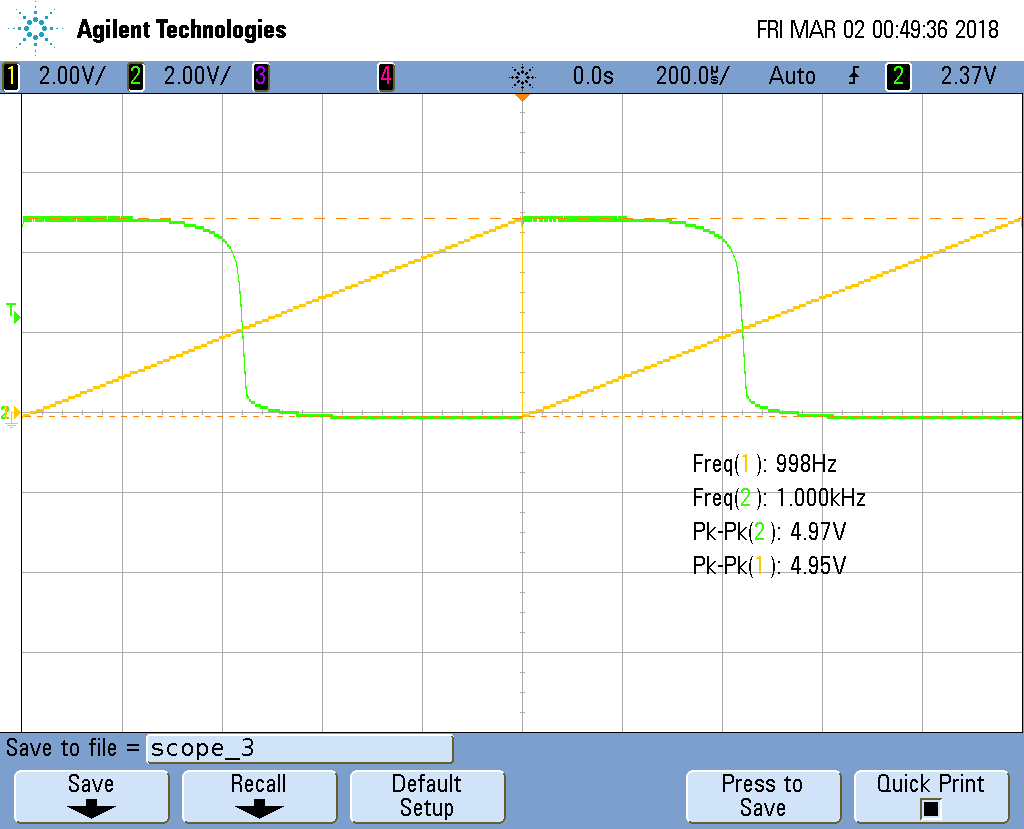
\includegraphics[scale=0.30]{./images/vout_and_vin_inverter_alt.png}
	\caption{$V_{out}$ and $V_{in}$}
	\label{fig:vout_and_vin_inverter_alt}
\end{figure}

\FloatBarrier

{\footnotesize $V_{out}$ versus time is in green. $V_{in}$ versus time is in yellow.}

\FloatBarrier

When the input voltage is low, the PMOS is turned on, pulling up $V_{out}$ to supply.
So, the output is high when the input is low.
When the input voltage is high, the NMOS is turned on, pulling down $V_{out}$ to ground.
Thus, the circuit acts as an inverter, explaining why the output transitions as it does.
The ramp function resets every period, which is why the output does the same.

\FloatBarrier

\begin{figure}[h!]
	\centering
	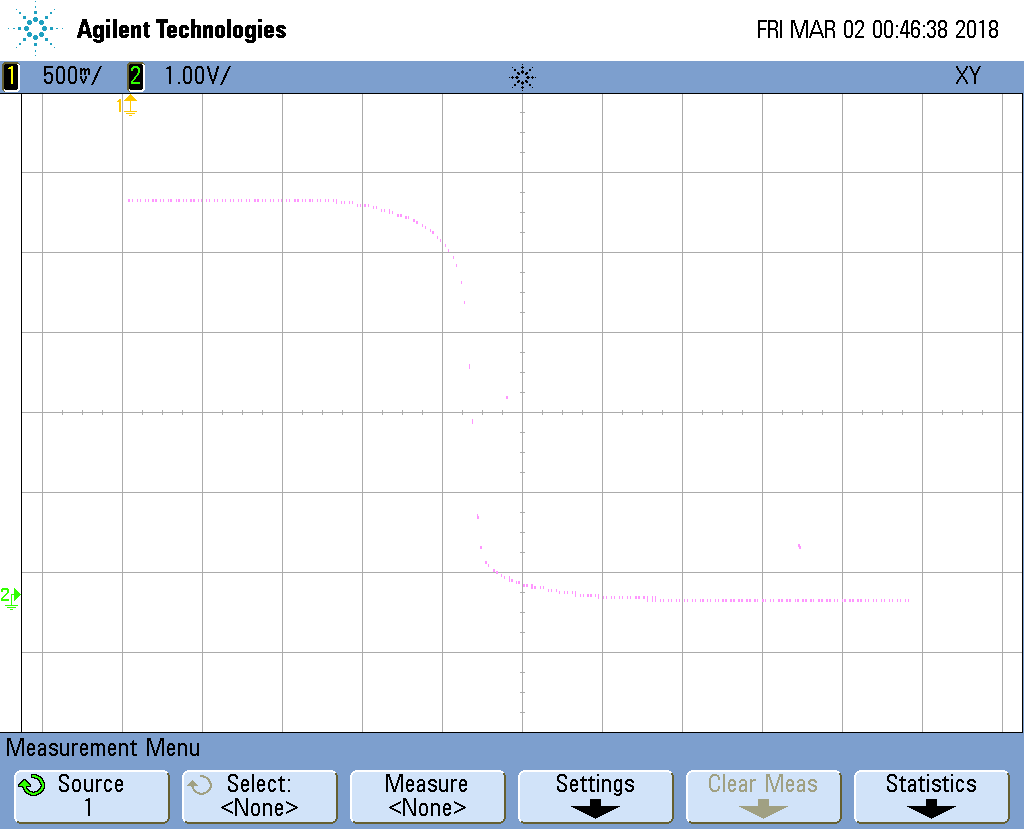
\includegraphics[scale=0.30]{./images/vtc.png}
	\caption{Voltage Transfer Characteristic of CMOS Inverter - $V_{out}$ versus $V_{in}$}
	\label{fig:vtc.png}
\end{figure}

\FloatBarrier

$V_{in}$ is a ramp function, meaning its range is simply from ground to supply.
So, when $V_{out}$ is plotted against $V_{in}$, the value of $V_{out}$ can be observed at every possible value at and between the high and low values.
Thus, the inverting voltage transfer characteristic of the CMOS inverter is observed in this plot.
The physics of why the inverter works in this manner is explained above.

\FloatBarrier

\begin{figure}[h!]
	\centering
	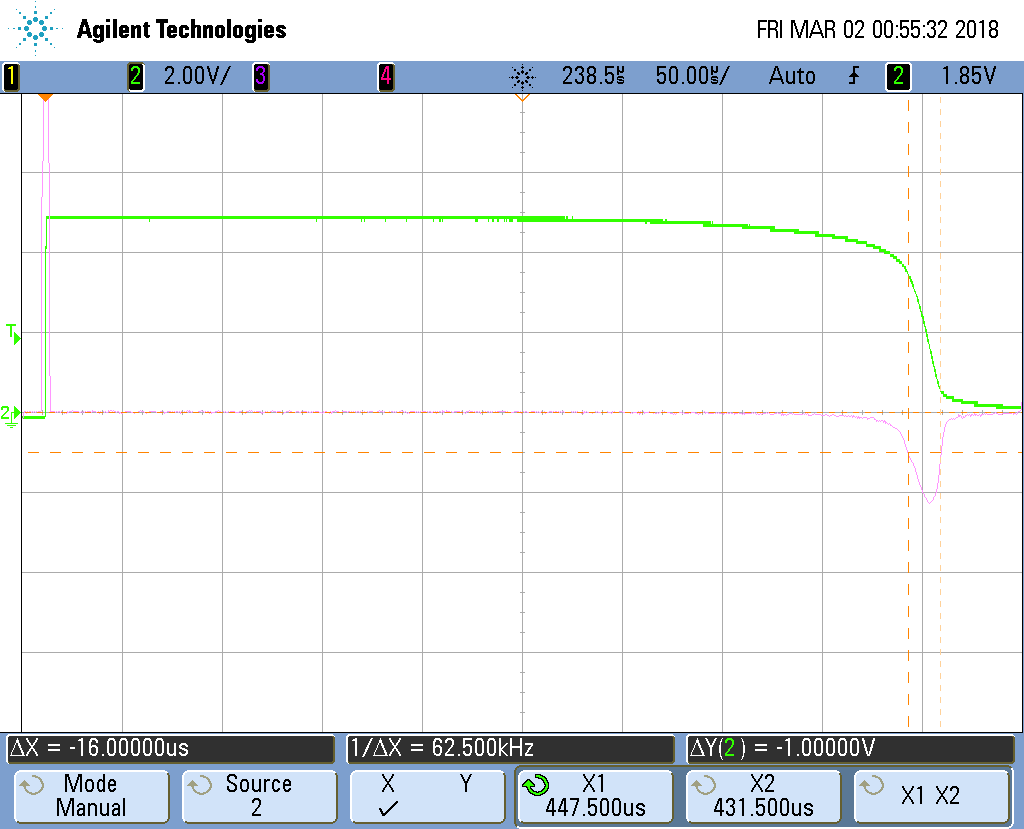
\includegraphics[scale=0.30]{./images/vil_vih_measure.png}
	\caption{$V_{IL}$ and $V_{IH}$ Measurement}
	\label{fig:vil_vih_measure}
\end{figure}

\FloatBarrier

{\footnotesize The green curve is $V_{out}$ versus time. The purple curve is $\frac{dV_{out}}{dV_{in}}$ versus time.}

\FloatBarrier

$V_{IL}$ and $V_{IH}$ are defined as the two points along the voltage transfer characteristic at which $\frac{dV_{out}}{dV_{in}} = -1$.
The points at which $\frac{dV_{out}}{dV_{in}}$ attains a value of $-1$ is where the $V_{IL}$ and $V_{IH}$ times are determined.

\FloatBarrier

\begin{table}[h!]
	\centering
	\caption{$V_{IL}$ and $V_{IH}$ Times}
	\label{tab:vil_vih_measure}
	\csvautotabular{./data/vil_vih_measure.csv}
\end{table}

\FloatBarrier

Table (\ref{tab:vil_vih_measure}) lists the times at which $V_{IL}$ and $V_{IH}$ are the values of $V_{in}$ relative to the start of the ramp function's period based on the measurements in table (\ref{fig:vil_vih_measure}).
With time as the independent variable and $V_{in}$ as the dependent variable, the starting point of the ramp function's period is the point ($0$\si{\micro\second},$0$\si{\volt}) and the ending point is ($1000$\si{\micro\second},$5$\si{\volt}).
This is because the period of the ramp function is given by the reciprocal of its frequency, $1$\si{\kilo\hertz}, and its maximum attainable value is the supply voltage, $5$\si{\volt}.
Therefore, the following equation describes $V_{in}$ as a function of time within one period:

\begin{equation}
	\label{eq:vin_vs_time}
	V_{in} = (0.005[\frac{V}{\mu s}])t \ , \ 0[\mu s] < t < 1000[\mu s]
\end{equation}

Using equation (\ref{eq:vin_vs_time}) and the times from table (\ref{tab:vil_vih_measure}), $V_{IL}$ and $V_{IH}$ can be computed.
The results are presented in table (\ref{tab:noise}).

\FloatBarrier

\begin{table}[h!]
	\centering
	\caption{Values Used for Noise Margin Calculations}
	\label{tab:noise}
	\csvautotabular{./data/noise.csv}
\end{table}

\FloatBarrier

The noise margins of a CMOS inverter are defined by:

\begin{equation}
	\label{eq:nml}
	NM_{L} = V_{IL} - V_{OL}
\end{equation}

\begin{equation}
	\label{eq:nmh}
	NM_{H} = V_{OH} - V_{IH}
\end{equation}

The values for the noise margins of this CMOS inverter are given in table (\ref{tab:noise_margins}).

\FloatBarrier

\begin{table}[h!]
	\centering
	\caption{Noise Margins}
	\label{tab:noise_margins}
	\csvautotabular{./data/noise_margins.csv}
\end{table}

\FloatBarrier

A square wave input with the same frequency and amplitudes is then provided to the CMOS inverter.

\FloatBarrier

\begin{figure}[h!]
	\centering
	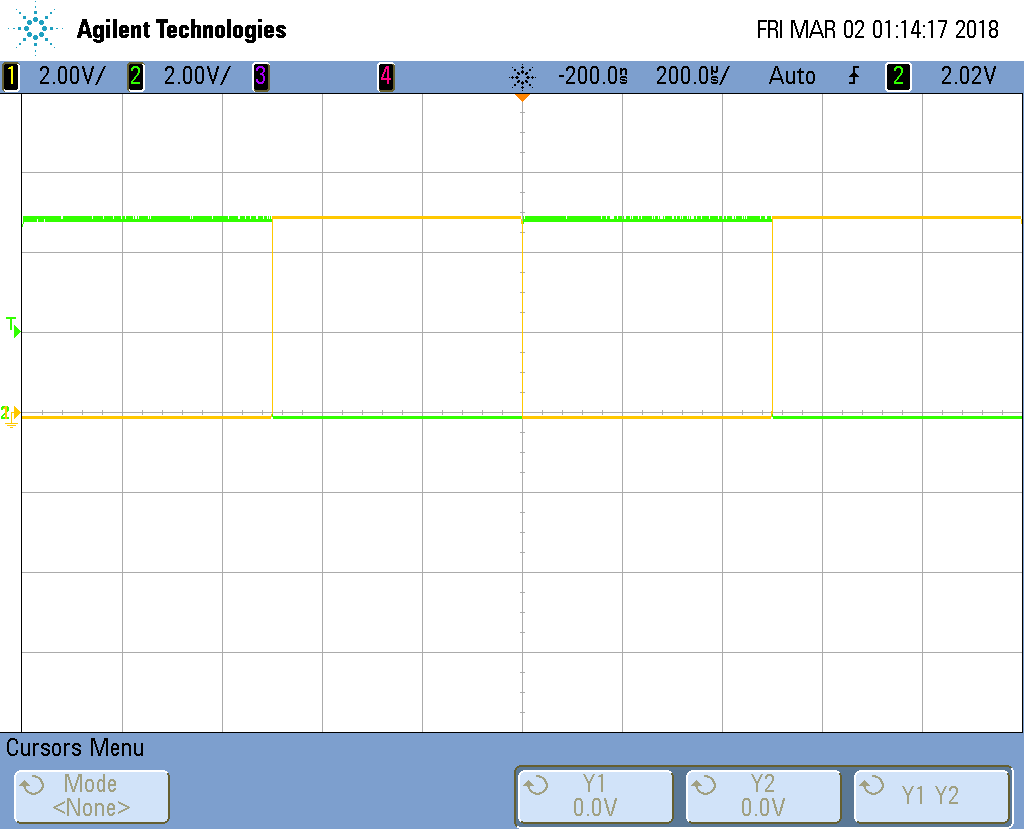
\includegraphics[scale=0.30]{./images/square_wave_inverter.png}
	\caption{Square Wave Input - Transient}
	\label{fig:square_wave_inverter}
\end{figure}

\FloatBarrier

{\footnotesize The same color convention as figure (\ref{fig:vout_and_vin_inverter_alt}) is followed.}

\FloatBarrier

\begin{figure}[h!]
	\centering
	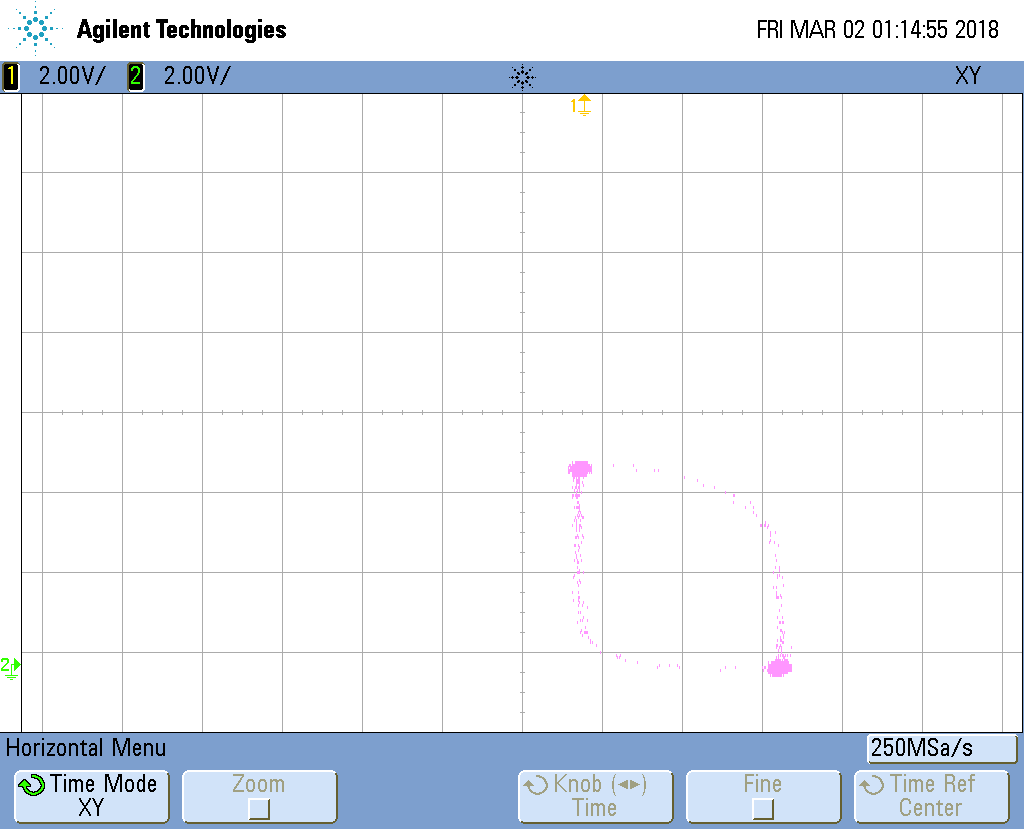
\includegraphics[scale=0.30]{./images/square_wave_vtc.png}
	\caption{Square Wave Input - Voltage Transfer Characteristic}
	\label{fig:square_wave_vtc}
\end{figure}

\FloatBarrier

The two points ( $V_{out}$ , $V_{in}$ ) at which the output is pulled to supply and ground are very pronounced in figure (\ref{fig:square_wave_vtc}).
However, because the square wave transitions so quickly, very few other points between are sampled.
As a result, the quality of the voltage transfer characteristic is significantly diminished.
A sine wave input is then tested.

\FloatBarrier

\begin{figure}[h!]
	\centering
	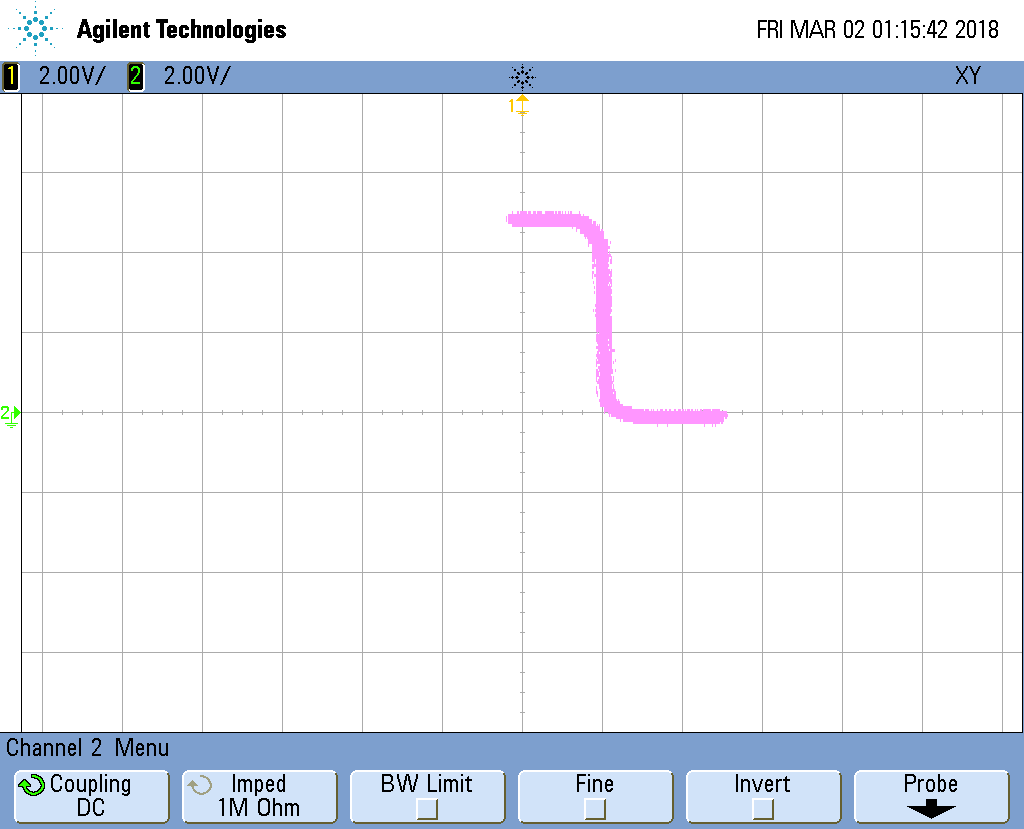
\includegraphics[scale=0.30]{./images/sine_wave_input_vtc.png}
	\caption{Sine Wave Input - Voltage Transfer Characteristic}
	\label{fig:sine_wave_input_vtc}
\end{figure}

\FloatBarrier

In the same period, the sine wave gives much better quality than the ramp function input when determining the voltage transfer characteristic.
